\subsection{Солнечные и лунные затмения. Сарос}
\subsubsection{Полное солнечное затмение}
Диаметр тени спутника при полном центральном затмении (когда центры трёх тел лежат на одной прямой), с большой точностью равен: 
\begin{equation}
d_\text{тени} = 2 \cdot \frac{R_{\moon}(a - R_\oplus) - R_\odot \left( a - R_\oplus \right)}{a - a_{\moon}},
\end{equation}
где $R_{\moon}$~--- радиус Луны, 
$R_\oplus$~--- радиус Земли, 
$R_\odot$~--- радиус Солнца, 
$a$~--- расстояние от Земли до Солнца, 
$a_{\moon}$ --- расстояние от Земли до Луны.

Среднее значение  этой величины около 200 км, максимальное около 215 км. При нецентральном затмении максимальный диаметр тени Луны на поверхности Земли может достигать 270~км (Рис.\,\ref{fig:eclipses-full-solar-eslipse}).

\begin{figure}[h!]
\centering
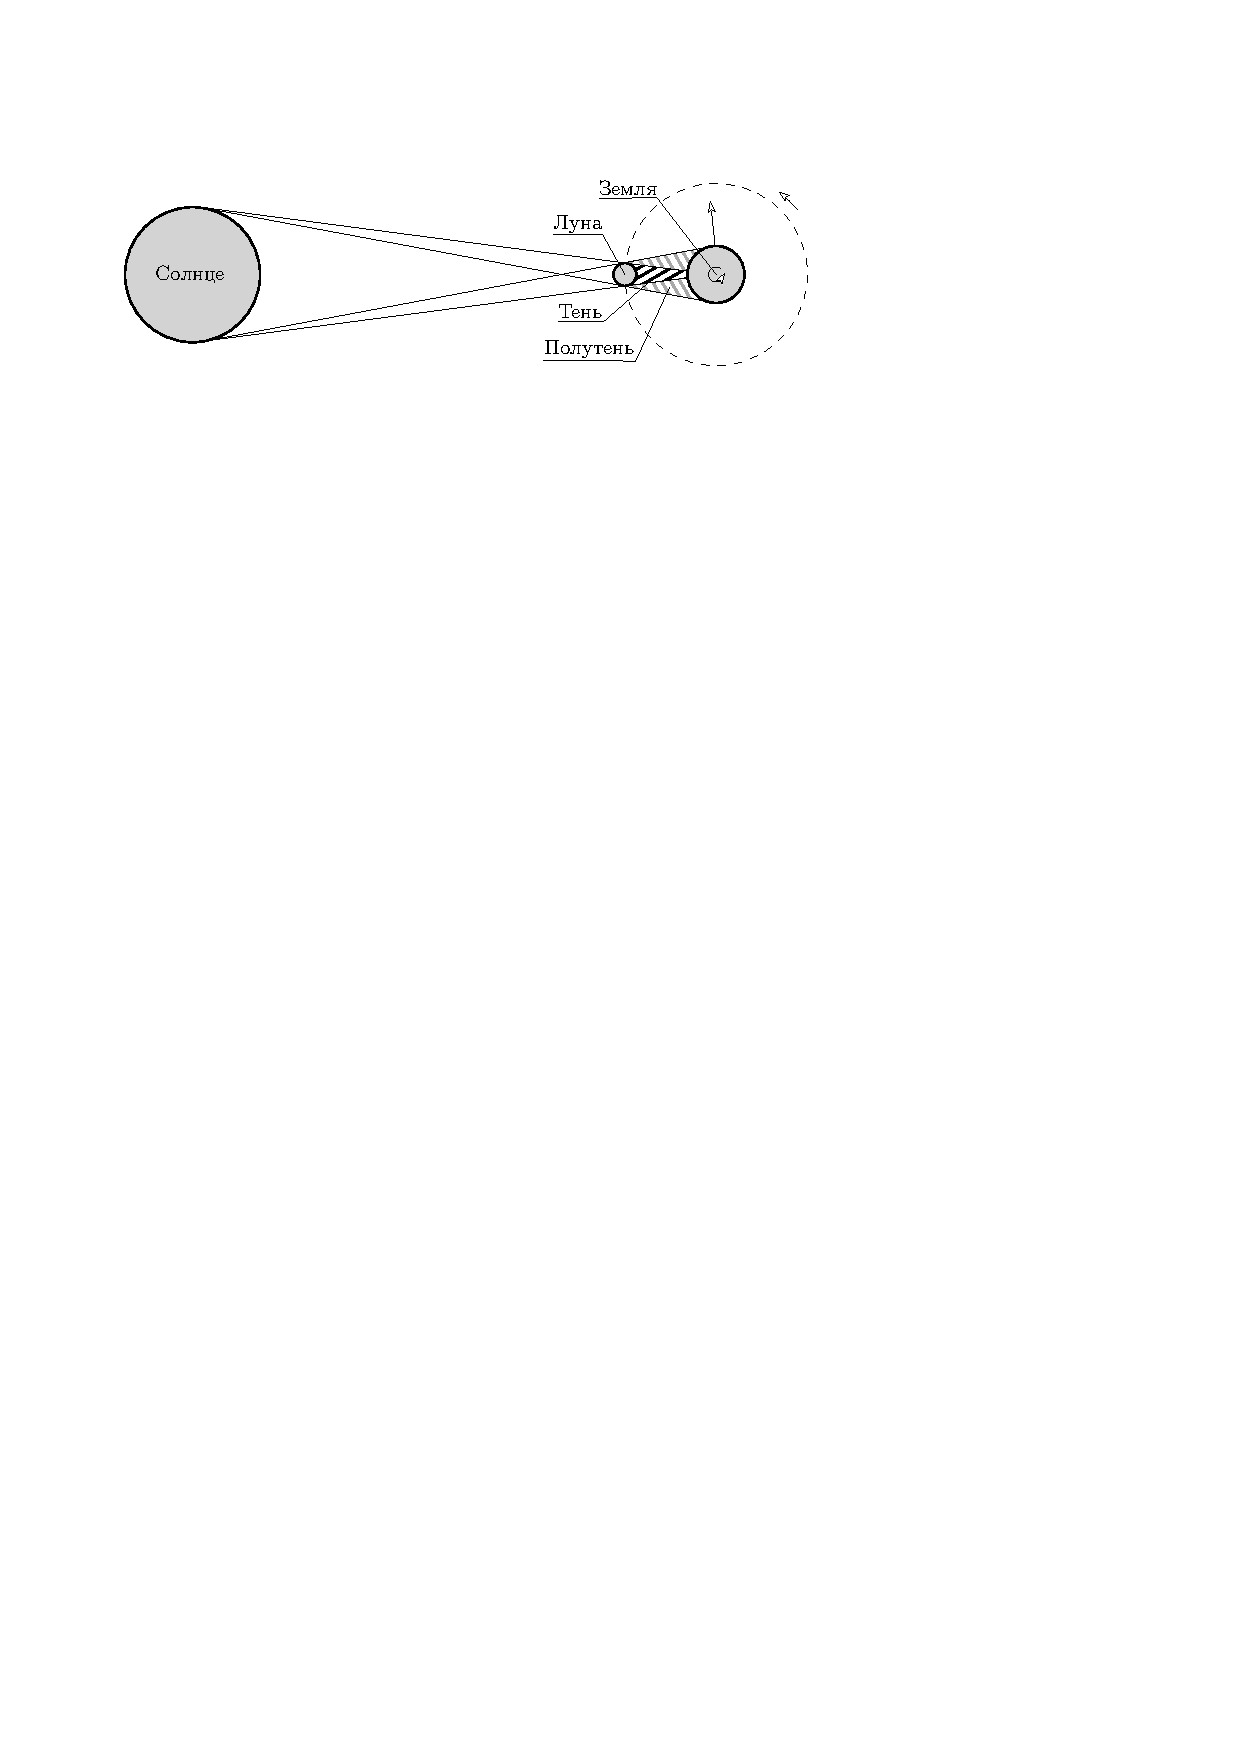
\includegraphics[width = .8\textwidth]{full_eclipse}
\caption{Полное солнечное затмение}
\label{fig:eclipses-full-solar-eslipse}
\end{figure}

При \term{кольцеобразном солнечном затмении} Луна относительно Земли расположена так, что конус её тени не достаёт до поверхности планеты, и вокруг Луны можно наблюдать яркое кольцо незакрытой части солнечного диска (Рис.~\ref{fig:eclipses-circle-solar-eslipse}).
\begin{figure}[h!]
	\centering
	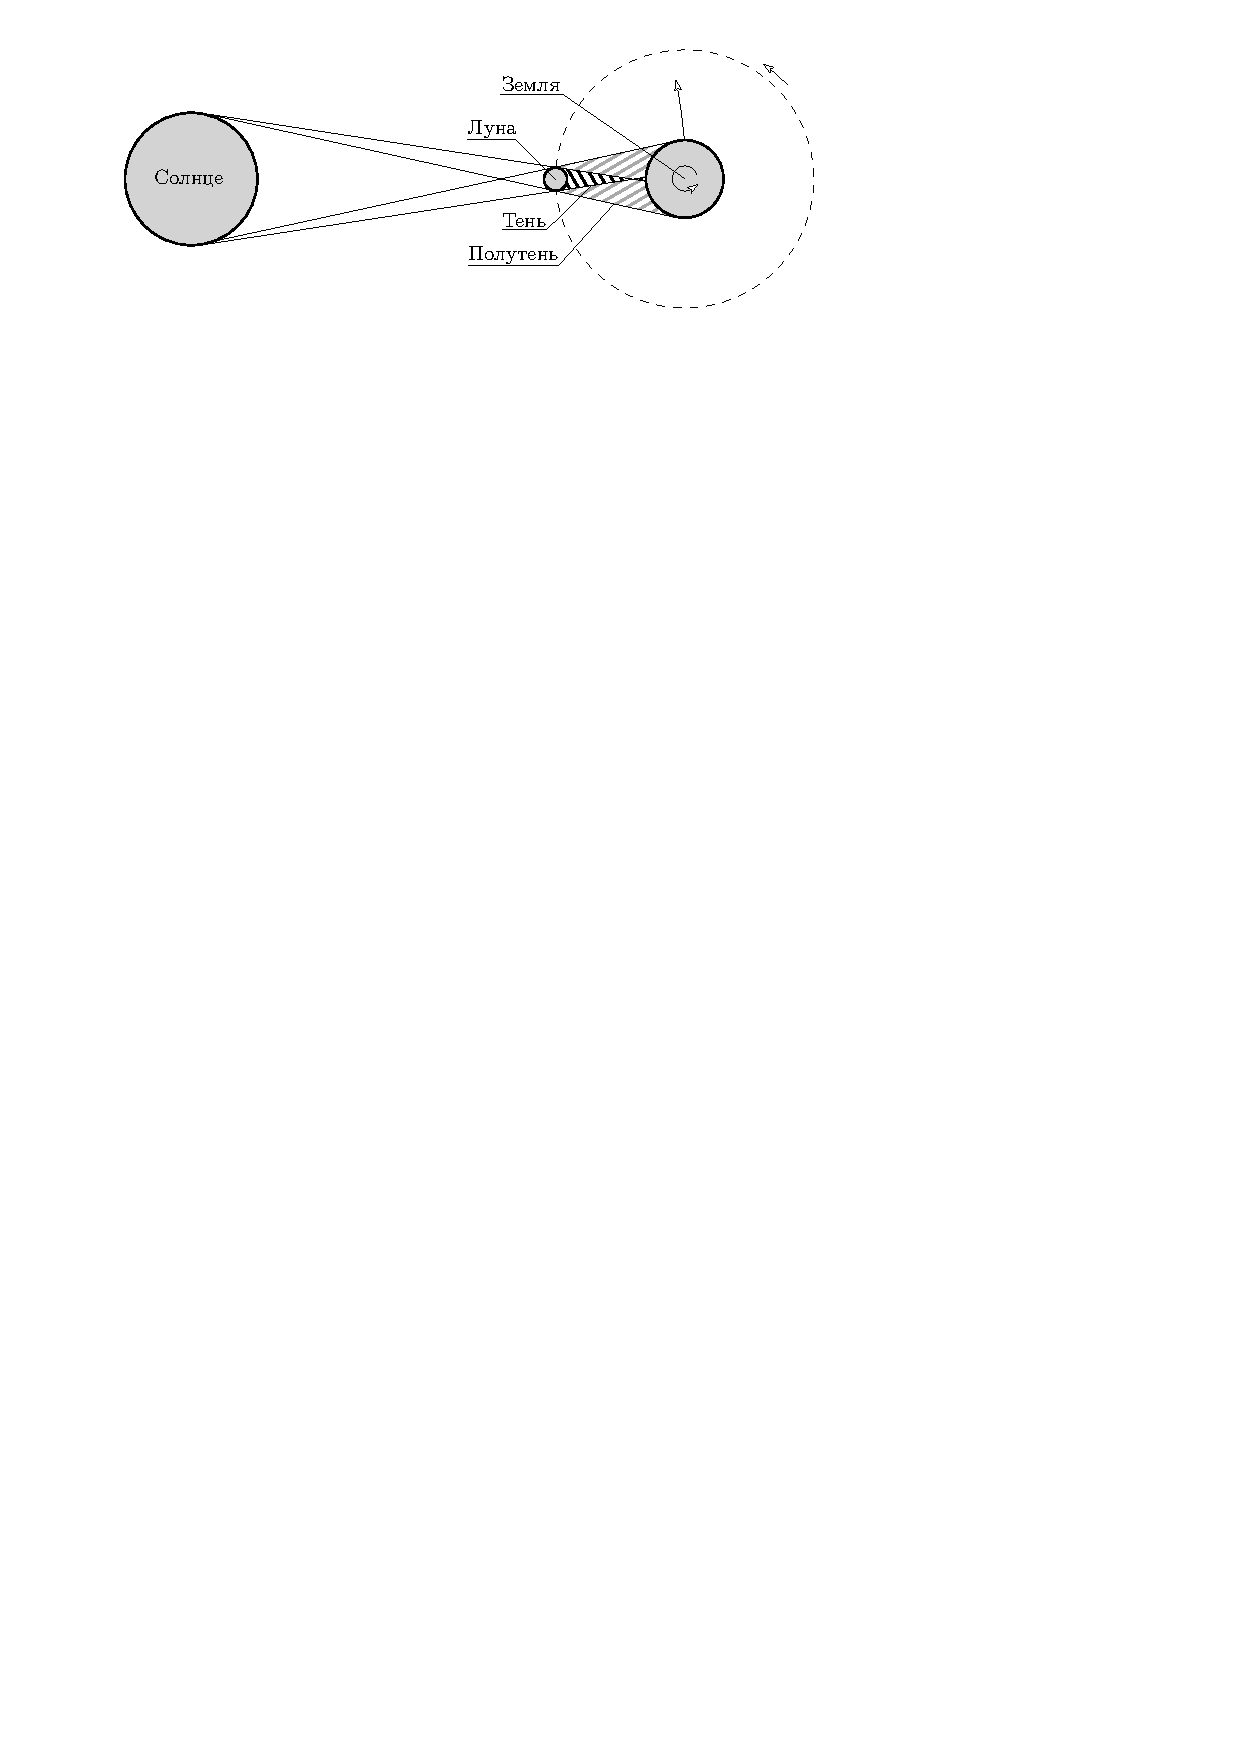
\includegraphics[width = 0.95\textwidth]{partly-eclipse}
	\caption{Кольцеобразное солнечное затмение}
	\label{fig:eclipses-circle-solar-eslipse}
\end{figure}

\term{Лунное затмение} в отличие от солнечного, видно со всего ночного полушария. Диаметр земной тени на расстоянии Луны превышает размер последней примерно в 2.5-3 раза (Рис.\,\ref{fig:moon-eclipse-scheme}).

\term{Синодический месяц}~--- промежуток времени между одинаковыми фазами Луны. Он равен 29.53 суток.

\term{Драконический месяц}~--- промежуток времени между двумя последовательными прохождениями Луны через один и тот же узел орбиты. Драконический месяц равен 27.21 суток.

\term{Сарос}~--- промежуток  времени, по прошествии которого солнечные и 
лунные затмения повторяются в прежнем порядке. Сарос составляет ровно 242 драконических месяца или 223 синодических месяца. Таким образом, его продолжительность примерно 18 лет 11 дней 8 часов.

\begin{figure}[h!]
\centering
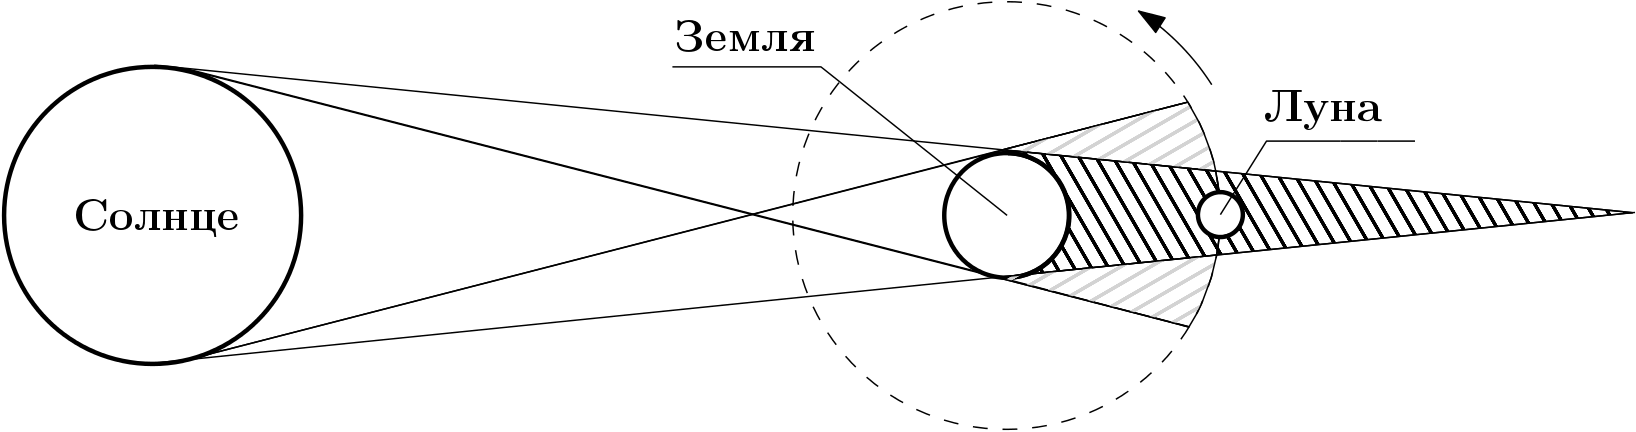
\includegraphics[scale=0.27]{moon-eclipse}
\caption{Схема лунного затмения}
\label{fig:moon-eclipse-scheme}
\end{figure}

\begin{wrapfigure}[9]{r}{.5\tw}
	\centering
	\vspace{-1pc}
	\includegraphics[width = 0.24\textwidth]{phases}
	\hfill
	\includegraphics[width = 0.24\textwidth]{phases-2}
	\caption{Частное и полное затмение}
	\label{fig:part-eclipses-scheme}
\end{wrapfigure}
Важной характеристикой любого затмения является его \term{фаза}~--- отношение закрытой части диаметра затмеваемого тела, проходящей через центр затмевающего тела, к полному диаметру затмеваемого тела. Для полного затмения эта величина рассчитывается немного иначе. Для Луны затмевающим <<телом>> является тень Земли. Фазу частного и полного затмения можно вычислить по следующим формулам (см.~Рис.\,\ref{fig:part-eclipses-scheme}):\begin{equation}
\Phi_{\text{част}} = \frac{x}{D}, \quad \quad \quad \Phi_{\text{полн}} = 1 + \frac{d}{D},
\end{equation}
где $D$~--- диаметр затмеваемого тела.

Иногда вводят такое понятие, как \term{площадная фаза затмения}, т.е. отношение площади закрытой части диска затмеваемого диска к полной площади его диска. Чаще всего  площадную фазу используют применительно к двойным звёздам, когда считают падение блеска при затмении одной звезды другой.
